\chapter{$\gamma$-Astronomie} 
Die Astronomie ist die Wissenschaft des Universums und beschreibt die Bewegung und Eigenschaften von Himmelskörpern wie Planeten oder Galaxien, interstellarer Materie und Strahlung. Betrachtete man frueher nur Licht im optisch sichtbaren Bereich, so sind im 20. Jahrhundert einige zusatliche Quellen dazugekommmen. Dazu zaehlen die von Viktor HESS durch Ballonversuche entdeckte kosmische Strahlung, die Roentgen-/bzw die Gammastrahlung sowie die Neutrinoastronomie. Die Gammaastronomie beschaftigt sich mit Photonen im Bereich von bis . Photonen haben den Vorteil, dass sie nicht wie geladene Teilchen durch elektromagnetische Felder abgelenkt werden und somit ihre Quelle leichter detektiert werden kann. Zudem sind sie auch noch deutlich leichter zu detektieren sind als Neutrinos. Da die Energie dieser Photonen so hoch ist, koennen sie nicht thermischen Ursprungs sein sondern kommen aus anderen Quellen, deren Untersuchung das Ziel der Hochenergie-Gamma-Astronomie ist.

%cite Design concept

\section{Entstehung hochenergetischer Strahlung}

\begin{description}
\item[inverser Comptoneffekt]\hfill \\
Durch den Comptoneffekt koennen hochenergetische Photonen einen Teil ihres Impulses und Energie an ein freies Elektron uebergeben. Dieser Prozess kann auch invers ablaufen und somit kann ein niederenergetisches Photon, zum Beispiel aus dem kosmischen Mikrowellenhintergrund (E), durch einen Stoss mit einem Elektron eine hohe Energie bekommen.
\item[Zerfall von schweren Teilchen]\hfill \\ 
Zerfallen schwerere Teilchen in Photonen, so wird die Ruheenergie dieses Teilchens in kinetische Energie der Photonen umgewandelt. Ein Beispiel hierfuer ist der Zerfall des neutralen Pions, die haufig bei der Kollision von Atomkernen entstehen. Das Pion hat eine Ruhemasse von 135MeV \cite{PDG} und zerfaellt fast ausschliesslich in zwei Photonen, die dann eine Energie von ungefaehr 68 MeV haben.
\item[Materie-Antimaterie-Annihilation]\hfill \\
Bei der Kollision von Materie mit Antimaterie vernichten sich die beiden Teilchen und es entstehen Neue. Dies koennen Photonen sein oder Teichen, die wiederum in Photonen zerfallen. Ein prominetes Beispiel hierfuer ist die Elektron-Positron-Annihilation. Besitzen die beiden Teilchen keine kinetische Energie, so zerfallen sie in zwei Photonen mit der Energie E=511keV.
\item[Bremstrahlung]\hfill \\
Durchfliegen hochenergetische Teilchen Materie, so kann es vorkommen, dass diese eng an den Atomen vorbeifliegen und abgelenkt werden. Durch diese Ablenkung werden Photonen abgestrahlt.
\end{description}

\section{Quellen hochenergetischer Strahlung}
Ziel VHE-Astronomie ist es die Quellen hochenergetischer Gammastrahlung zu erforschen. Folgende Quellen sind bekannt:

\begin{description}
\item[Schwarze Loecher]\hfill \\
Schwarze Loecher sind Ueberreste von Supernovae massiver Sterne -> aktive Kerne
\item[Supernova Uebereste]\hfill \\
Supernovae
\item[Pulsare]\hfill \\
Kollabieren die Überreste einer Supernova von einem Durchmesser von ca $10^6km$ auf ca $20km$ ensteht ein Neutronenstern, der sich aufgrund der Drehimpulserhaltung sehr schnell dreht. Solche Konstrukte nennt man Pulsare. Durch die schnelle Rotation entstehen starke elektromagnetische Felder, die geladene Partikel beschleunigen können. Pulsare strahlen ungefähr $10^42eV/s$ ab.
\item[Binäre Systeme]\hfill \\ 
Befindet sich ein Neutronenstern oder Pulsar in einem System mit einem normalen Stern, entsteht durch absaugen von Materie eine Akkretitionsscheibe um den Neutronenstern beziehungsweise um den Pulsar. Da die Materie in diesem System durch Gravitation beschleunigt wird, werden Energien der Größenordnung $10^19 eV$ erzeugt. 
\item[Dunkle Materie]\hfill \\
Hochenergetische Photonen koennen auch nach Prinzipien erzeugt werden, die man heute noch nicht versteht. So koennte es moeglich sein, dass hochenergetische Photonen durch den Zerfall von Partikeln der dunklen Materie stammen. Die Supersymmetrie sagt zum Beispiel den Zerfall von schweren WIMPS in Photonen vorraus. Durch Detektion solcher Ereignisse liesse sich auf neue Physik schliessen.
\end{description}


\section{Detektion von Strahlung}
Prinzipiell laesst sich zwischen bodengestuetzter und satellitengestuetzter Gammaastronomie unterscheiden. Durch den Einsatz von Satelliten vermeidet man den stoerenden Einfluss der Erdatmosphaere, muss dafuer Abstriche in der Groesse der Detektoren machen und mit hohen Kosten kalkulieren. Hier soll sich nur mit der bodengestuetzten Variante beschaeftigt werden.

\subsection{Luftschauer}
Treten hochenergetische Photonen in die Materie ein, so wechselwirken sie mit dieser ueber Paarbildung. Das entstehende Elektron bzw Positron verliert daraufhin Energie durch Bremstrahlung, worauf die entstehenden Photonen wieder durch Paarbildung wechselwirken koennen. Somit steigt die Anzahl der Teilchen exponentiell an und die durchschnittliche Energie nimmt exponentiell ab, bis die Teilchen ioniserend sind und der Schauer verschwindet. Die entstehenden Teilchen lassen sich nicht direkt nachweisen, da der Schauer bereits in einer Hoehe von ca 10km verschwindet. %bild zur veranschaulichung
Neben elektromagnetischen Schauern existieren noch hadronische und myonische Schauer. Hadronische Schauer entstehen wenn hochenergetische Hadronen in die Atmosphaere eindringen. Durch die Wechselwirkung von Hadronen entstehen haufig Pionen, die wiederum in Photonen zerfallen, wodurch wiederum ein elekromagnetischer Schauer entsteht, der allderdings einen anderen Ursprung hat. Entstehen Myonen in einem Schauer, so besteht das Problem, dass diese kaum Energie abgeben und bei hoher Geschwindigkeit den Erdboden erreichen. Somit gibt nur ein Teil des Schauers die Energie ab und die Messung weicht von der Realitaet ab.

\subsection{Cherenkov Strahlung}
Cherenkov Strahlung tritt auf, wenn geladene sich Teilchen in Materie schneller als Photonen bewegen und lässt sich analog zum Überschallknall erklären. Das geladene Teilchen polarisiert auf seiner Trajektorie die einzelnen Atome, die somit Licht sphaerisch abstrahlen. Da sich das Teilchen allerdings schneller als das Licht bewegt, entsteht ein Kegel konstruktiver Interferenz. Somit entsteht ein Lichtblitz, der sich kegelfoermig mit dem Oeffnungswinkel %bild zur interferenz
\begin{equation}
\theta = \arccos\left(\frac{1}{\beta n}\right) \label{eq:cherenkow}
\end{equation}\\
ausbreitet. Fuer Luft (in Bodennaehe) ergibt sich somit ein maximaler Oeffnungswinkel von
\begin{figure}[htbp]
\centering
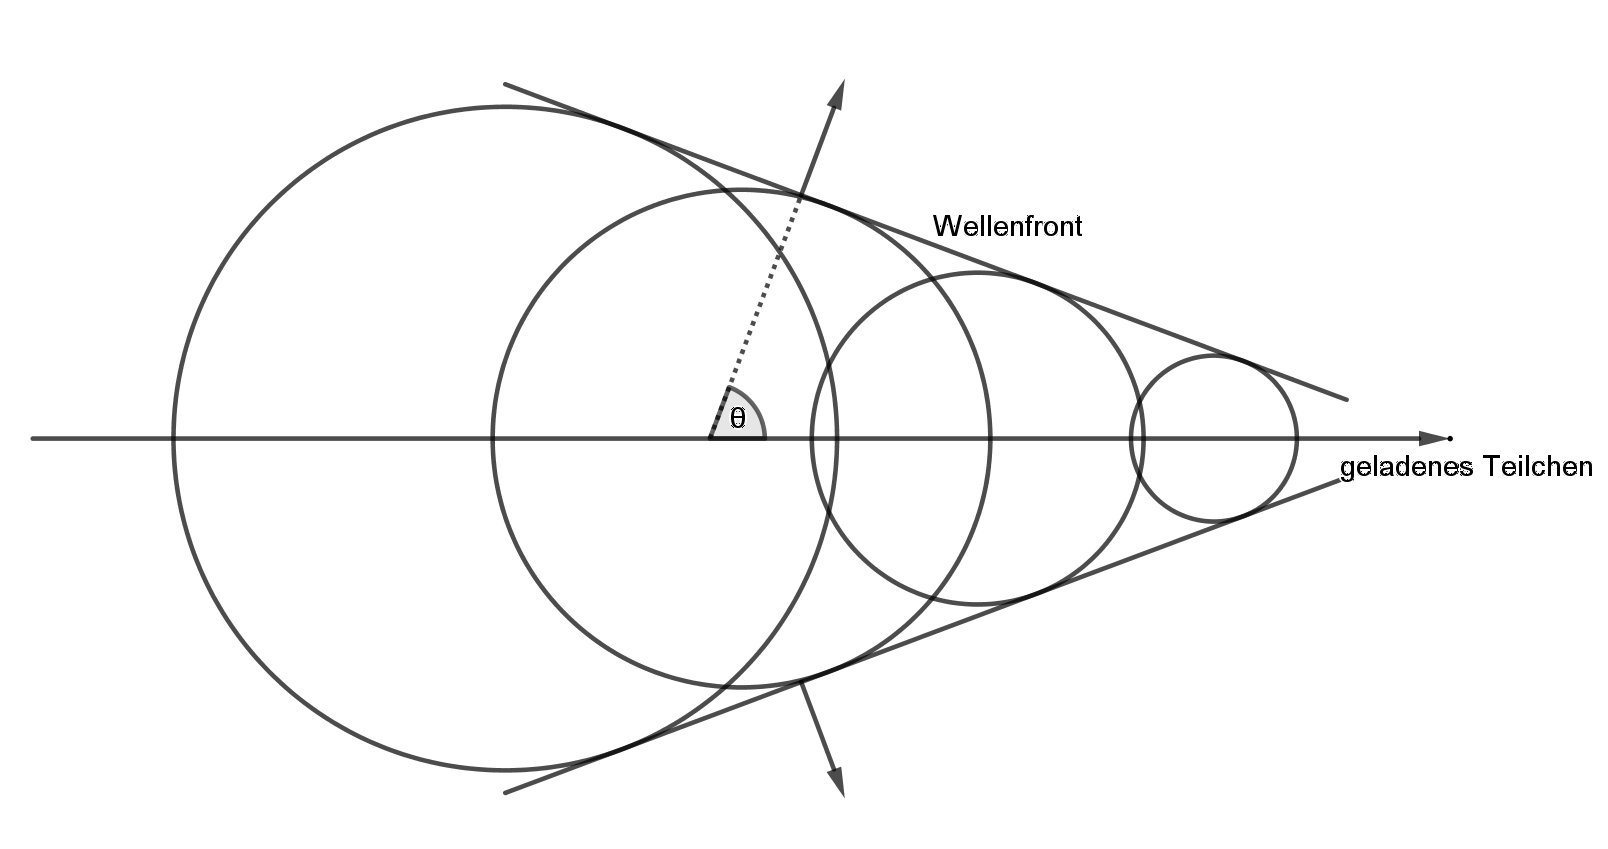
\includegraphics[width=0.7\textwidth]{Images/cherenkow.png}
\caption{Der Cherenkoweffekt: Ein geladenes Teilchen durchfliegt ein dielektrisches Medium und erzeugt Wellenfronten.}
\label{img:cherenkow}
\end{figure}

\subsection{Bodengestützte Detektion der Cherenkovstrahlung}
Da aufgrund der Atmosphaere weder das primaere Photon noch die Teilchen des Luftschauers detektiert werden koennen, versucht man die Cherenkovstrahlung, die durch den Luftschauer entsteht zu detektieren. Dazu muss eine grosse Flaeche abgedeckt werden, da selbst bei vertikaler Einstrahlung der Schauer einen Durchmesser von ca 250m haben kann %design concept 
Somit ergeben sich Flachen der Grossenordnung von $10^4-10^5 m^2$. Um diese Flaechen abdecken zu koennen, verwendet man Teleskope mit effektiven Flaechen von ungefaehr $100 m^2$ (VERITAS). Haufig bestehen die Reflektoren aus vielen einzelnen Spiegeln um die Kosten zu druecken. Im Brennpunkt der Spiegel befindet sich der Cherenkovdetektor der in der Regel aus vielen Photomultipliern (PMTs) besteht. Somit erhaelt man effektiv eine Kamera mit einer typischen Aufloesung von ca 2000 Pixeln. Die Aufloesung ist im Vergleich zu CCD Kameras einerseits eher gering, da die Cherenkov Kamera in der Lage sein muss einzelne Photonen zu detekieren und andererseites dauern Cherenkovschauer nur wenige Nanosekunden, die wiederum zeitlich aufgeloest werden muessen. Zusaetlich muessen die Teleskope elektromagenetische Schauer von hadronisches Schauern unterscheiden und duerfen nicht durch Hintergrundeffekte wie zum Beispiel Sternenlicht gestoert werden.

\begin{figure}[htbp]
\centering
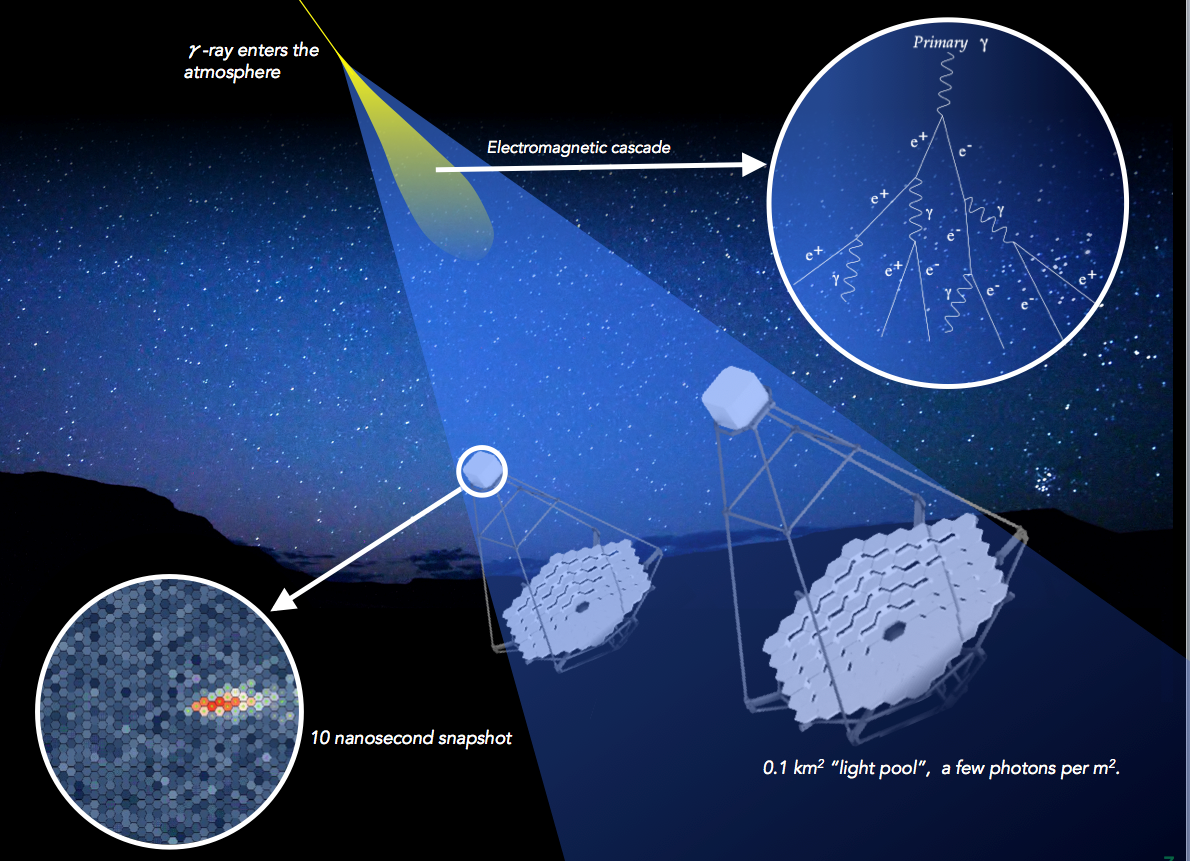
\includegraphics[width=\textwidth]{Images/detection.png}
\caption{Detektion hochenergetischer Strahlung}
\label{img:detection}
\end{figure}
